\chapter{Large-Scale Unconstrained Optimization Problems}
\label{chap:large-scale}

\section{Introduction}

Practical applications can involve hundreds or thousands of variables.
With the techniques from the previous chapters, we may be faced with high costs:
\begin{itemize}
    \item Computational costs (CPU time).
    \item Storage costs (memory).
\end{itemize}

In this chapter, we will present techniques to overcome these difficulties.

\section{Inexact Newton Methods}

In Newton methods, we find the direction $p_k^N$ by solving the linear system:
\[
    \nabla^2 f_k p_k^N = - \nabla f_k.
\]
(Formally, $p_k^N = - (\nabla^2 f_k)^{-1} \nabla f_k$).

\paragraph{Our goal} is to find an approximation $p_k$ of $p_k^N$ that is not too costly to compute: these are the inexact Newton methods.
For example, we can use iterative methods such as the conjugate gradient to solve the system approximately.

The quality of the approximation will determine the convergence properties.

\subsection{Local Convergence}

It is reasonable to stop solving the system $\nabla^2 f_k p_k^N = -\nabla f_k$ when the residual
\[
    r_k = \nabla^2 f_k p_k + \nabla f_k
\]
is small.

For instance, by using a \textbf{forcing sequence} $(\eta_k) \in (0, 1)^\mathbb{N}$ and stopping when:
\begin{equation}
    \| r_k \| \le \eta_k \| \nabla f_k \|.
\end{equation}

The two theorems in this subsection apply to all inexact Newton methods satisfying the above condition.
(Proofs: \textit{Dembo et al.})

\begin{theoreme}[Local convergence]
    Suppose that $\nabla^2 f(x)$ exists and is continuous in a neighborhood of a minimizer $x^\star$, with $\nabla^2 f(x^\star)$ positive definite.
    Let $x_{k+1} = x_k + p_k$ (where we assume a unit step $\alpha_k=1$ near the solution) where $p_k$ satisfies:
    \[
        \| r_k \| \le \eta_k \| \nabla f_k \|.
    \]
    Suppose that $\eta_k \le \eta$ for all $k$, where $\eta \in [0, 1)$.

    Then, if $x_0$ is sufficiently close to $x^\star$, the sequence $(x_k)$ converges to $x^\star$.
    Moreover, there exists a certain $\hat{\eta} \in (\eta, 1)$ such that:
    \[
        \| \nabla^2 f(x^\star) (x_{k+1} - x^\star) \| \le \hat{\eta} \| \nabla^2 f(x^\star) (x_k - x^\star) \|.
    \]
\end{theoreme}

\subsection{Rate of Convergence}

\begin{theoreme}[Rate of convergence]
    Suppose the conditions of the previous theorem hold, and that $(x_k)$ converges to $x^\star$.
    \begin{itemize}
        \item The convergence rate is \textbf{superlinear} if $\lim_{k \to \infty} \eta_k = 0$.
        \item If $\nabla^2 f$ is Lipschitz-continuous near $x^\star$ and if $\eta_k = O(\| \nabla f_k \|)$, then the convergence is \textbf{quadratic}.
    \end{itemize}
\end{theoreme}

\paragraph{Proof elements.}
We can show that:
\[
    \frac{\| \nabla f_{k+1} \|}{\| \nabla f_k \|} \le \eta_k + o(1).
\]
\begin{itemize}
    \item If $\eta_k \to 0$, then the gradient (and thus the iterates) converges superlinearly.
    \item If $\nabla^2 f$ is Lipschitz continuous, we have $\nabla f_{k+1} = O(\| \nabla f_k \|^2)$, which implies quadratic convergence.
\end{itemize}

\paragraph{Remarks.}
\begin{itemize}
    \item The choice $\eta_k = \min(0.5, \sqrt{\| \nabla f_k \|})$ provides a \textbf{superlinear} convergence.
    \item The choice $\eta_k = \min(0.5, \| \nabla f_k \|)$ provides a \textbf{quadratic} convergence.
    \item These results are local: we assumed that $x_0$ was close to $x^\star$ and that $\alpha_k = 1$.
\end{itemize}

\subsection{Newton-CG Methods with Line Search}

The system $\nabla^2 f_k p_k = - \nabla f_k$ is solved using the conjugate gradient (CG) method.
We must stop if we encounter a direction of negative curvature (i.e., if $\nabla^2 f_k$ is not positive definite).

\section{Limited-Memory Quasi-Newton Methods (L-BFGS)}

When the Hessian is not available at a reasonable cost (in time or storage), limited-memory Quasi-Newton methods are useful.
They replace the storage of $n \times n$ matrices with the storage of a limited number of vectors of size $n$.
Here we focus on the \textbf{L-BFGS} (Low-storage BFGS) method, which stores the curvature information from the $m$ previous iterations.
(Derivation: \textit{\cite{nocedal1980updating}}).

\subsection{Review of BFGS}

The BFGS steps are $x_{k+1} = x_k - \alpha_k H_k \nabla f_k$, where $H_k$ is updated according to:
\begin{equation}
    H_{k+1} = V_k^\top H_k V_k + \rho_k s_k s_k^\top,
\end{equation}
with $V_k = I - \rho_k y_k s_k^\top$ and $\rho_k = \frac{1}{y_k^\top s_k}$.
We denote $s_k = x_{k+1} - x_k$ and $y_k = \nabla f_{k+1} - \nabla f_k$.

\subsection{Principles of L-BFGS}

\begin{itemize}
    \item Instead of storing the dense matrix $H_k$, we store $m$ vector pairs $(s_i, y_i)$.
    \item At each iteration, we replace the oldest pair $(s_{k-m}, y_{k-m})$ with the new one $(s_k, y_k)$.
    \item In practice, $m$ is chosen between 3 and 20.
    \item At iteration $k$, we have the current iterate $x_k$ and the pairs $(s_i, y_i)$ for $i = k-m, \dots, k-1$.
    \item We choose an initial approximation $H_k^0$.
\end{itemize}

\begin{figure}[htbp]
\centering
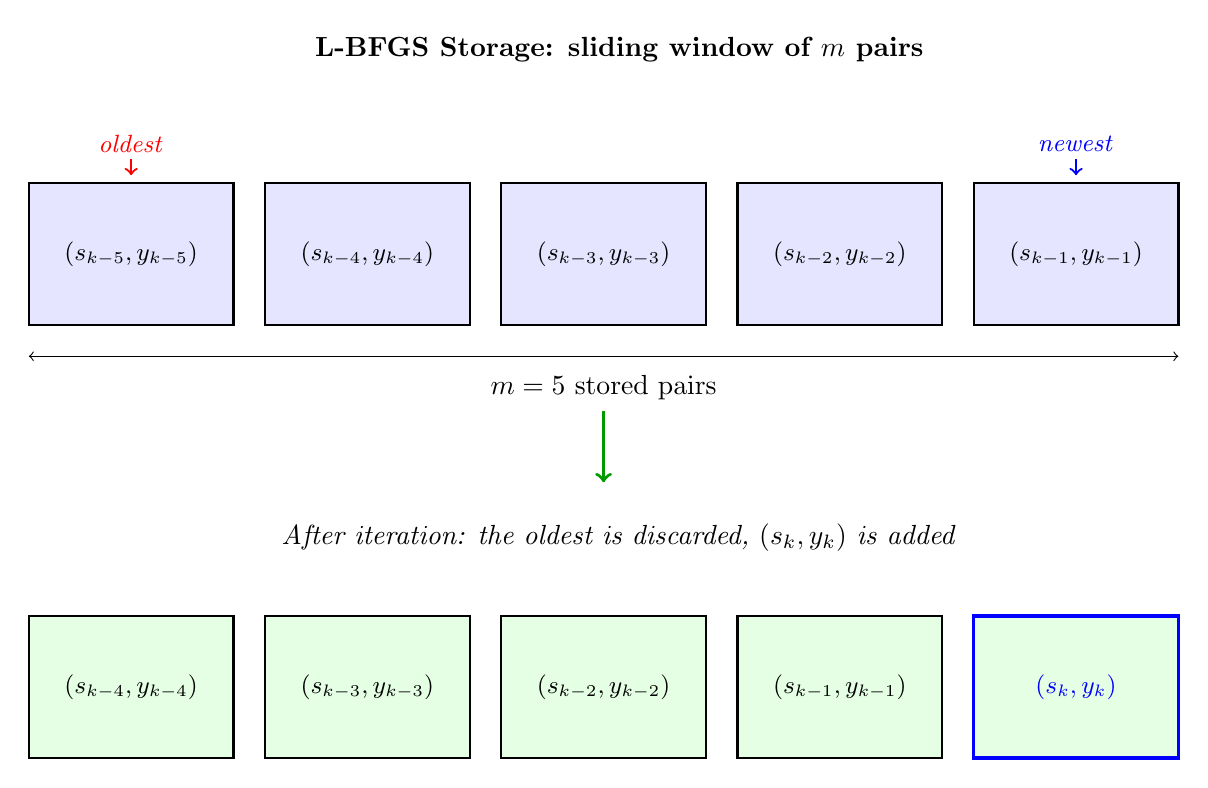
\begin{tikzpicture}[scale=1.0]
    % Title
    \node at (7.5, 3.5) {\textbf{L-BFGS Storage: sliding window of $m$ pairs}};
    
    % Memory slots (boxes) - wider spacing
    \foreach \i in {0,...,4} {
        \draw[thick, fill=blue!10] (\i*3, 0) rectangle (\i*3+2.6, 1.8);
    }
    
    % Labels for stored pairs - use smaller subscripts
    \node[font=\small] at (1.3, 0.9) {$(s_{k-5}, y_{k-5})$};
    \node[font=\small] at (4.3, 0.9) {$(s_{k-4}, y_{k-4})$};
    \node[font=\small] at (7.3, 0.9) {$(s_{k-3}, y_{k-3})$};
    \node[font=\small] at (10.3, 0.9) {$(s_{k-2}, y_{k-2})$};
    \node[font=\small] at (13.3, 0.9) {$(s_{k-1}, y_{k-1})$};
    
    % Oldest label
    \node[red, font=\small] at (1.3, 2.3) {\textit{oldest}};
    \draw[->, red, thick] (1.3, 2.1) -- (1.3, 1.9);
    
    % Newest label  
    \node[blue, font=\small] at (13.3, 2.3) {\textit{newest}};
    \draw[->, blue, thick] (13.3, 2.1) -- (13.3, 1.9);
    
    % m label at bottom
    \draw[<->] (0, -0.4) -- (14.6, -0.4);
    \node at (7.3, -0.8) {$m = 5$ stored pairs};
    
    % Vertical arrow between states - positioned after label
    \draw[->, very thick, green!60!black] (7.3, -1.1) -- (7.3, -2.0);
    
    % New state after update - more vertical space
    \begin{scope}[shift={(0, -5.5)}]
        \node at (7.5, 2.8) {\textit{After iteration: the oldest is discarded, $(s_k, y_k)$ is added}};
        
        \foreach \i in {0,...,4} {
            \draw[thick, fill=green!10] (\i*3, 0) rectangle (\i*3+2.6, 1.8);
        }
        
        \node[font=\small] at (1.3, 0.9) {$(s_{k-4}, y_{k-4})$};
        \node[font=\small] at (4.3, 0.9) {$(s_{k-3}, y_{k-3})$};
        \node[font=\small] at (7.3, 0.9) {$(s_{k-2}, y_{k-2})$};
        \node[font=\small] at (10.3, 0.9) {$(s_{k-1}, y_{k-1})$};
        \node[blue, font=\small\bfseries] at (13.3, 0.9) {$(s_k, y_k)$};
        
        % New pair highlight
        \draw[blue, very thick] (12, 0) rectangle (14.6, 1.8);
    \end{scope}
\end{tikzpicture}
\caption{Principle of L-BFGS storage: sliding window of $m$ pairs $(s_i, y_i)$. At each iteration, the oldest pair is eliminated and the new pair is added.}
\label{fig:lbfgs-storage}
\end{figure}

\begin{figureexplanation}
Figure~\ref{fig:lbfgs-storage} illustrates the storage principle of L-BFGS. Instead of maintaining the matrix $H_k$ (of size $n \times n$), we only keep the last $m$ pairs of vectors $(s_i, y_i)$. This approach reduces the storage cost from $O(n^2)$ to $O(mn)$, which is essential for large-scale problems.
\end{figureexplanation}

We can unroll the update formula recursively:
\begin{align*}
    H_k &= V_{k-1}^\top H_{k-1} V_{k-1} + \rho_{k-1} s_{k-1} s_{k-1}^\top \\
    &= V_{k-1}^\top (V_{k-2}^\top H_{k-2} V_{k-2} + \rho_{k-2} s_{k-2} s_{k-2}^\top) V_{k-1} + \rho_{k-1} s_{k-1} s_{k-1}^\top \\
    &= \dots \\
    &= (V_{k-1}^\top \dots V_{k-m}^\top) H_k^0 (V_{k-m} \dots V_{k-1}) \\
    &\quad + \rho_{k-m} (V_{k-1}^\top \dots V_{k-m+1}^\top) s_{k-m} s_{k-m}^\top (V_{k-m+1} \dots V_{k-1}) \\
    &\quad + \dots + \rho_{k-1} s_{k-1} s_{k-1}^\top.
\end{align*}

This formula allows computing the product $H_k \nabla f_k$ without ever forming the matrix $H_k$ (see Algorithm~\ref{alg:lbfgs-twoloop}, \textit{two-loop recursion}).

\paragraph{Complexity.}
Algorithm~\ref{alg:lbfgs-twoloop} requires $4mn$ operations, plus the cost of computing $H_k^0 q$ ($n$ multiplications if $H_k^0$ is diagonal).

\paragraph{Choice of $H_k^0$.}
In practice, choosing $H_k^0 = \gamma_k I$ with:
\begin{equation}
    \gamma_k = \frac{s_{k-1}^\top y_{k-1}}{y_{k-1}^\top y_{k-1}},
\end{equation}
gives satisfactory results. One can show that $\gamma_k$ roughly approximates one of the eigenvalues of the Hessian.

\paragraph{Line Search.}
As for BFGS, we use the (strong) Wolfe conditions and initialize the line search with $\alpha_k = 1$.

\bigskip
\begin{checkpoint}
\begin{itemize}
    \item \textbf{Inexact Newton:} What is the stopping criterion for solving the linear system?
    \item \textbf{Newton-CG:} Why is this method suitable for high dimensions (Matrix-vector products only)?
    \item \textbf{Negative Curvature Condition:} What does Newton-CG do if $p^T \nabla^2 f p < 0$?
\end{itemize}
\end{checkpoint}
